\documentclass{article}

\usepackage{times}
\usepackage{geometry}
\geometry{a4paper,left=0.6cm,right=0.7cm,top=1.5cm,bottom=1cm,columnsep=0.8cm}

\usepackage{fontawesome}          % icônes de base seulement
\usepackage[hidelinks]{hyperref}
\usepackage{multicol}
\usepackage{tikz}
\usepackage{hyphsubst}
\usepackage{moresize}
\usepackage{hyphenat}
\usepackage{tabularx}
\usepackage{xcolor}
\usepackage{enumitem}
\usetikzlibrary{calc, positioning}
\newcolumntype{Y}{>{\RaggedRight\arraybackslash}X}

% icônes manquantes -> puce
\makeatletter
\@for\sym:=faBrain,faMicrochip,faHandshakeO,faTools,faNetworkWired,%
             faDatabase,faServer,faGit,faUsers,faComments,faCalendar,faGroup\do{%
  \@ifundefined{\sym}{\expandafter\newcommand\csname\sym\endcsname{\textbullet}}{}}
\makeatother

% couleurs
\definecolor{maincolor}{HTML}{f0fafc}
\definecolor{seccolor}{HTML}{ffffff}
\definecolor{gray}{HTML}{8c94a9}
\definecolor{sidetext}{HTML}{59cee5}

% bande latérale bleue
\usepackage{eso-pic}
\AddToShipoutPictureBG{%
  \begin{tikzpicture}[remember picture,overlay]
    \fill[maincolor] (current page.north west) rectangle
                     ([xshift=0.3\paperwidth] current page.south west);
  \end{tikzpicture}%
}

% listes
\setlist[itemize]{itemsep=-2pt,topsep=0pt,leftmargin=1.08cm}
\renewcommand{\labelitemi}{\textcolor{sidetext}{\footnotesize$\bullet$}}

\setlength{\parindent}{0pt}
\usepackage{paracol}
\columnratio{0.3}

\begin{document}
\pagestyle{empty}

\begin{paracol}{2}
% ────────────────────────────────────────
% Colonne gauche
% ────────────────────────────────────────
\color{sidetext}
\vspace*{-0.5cm}

\noindent
\begin{minipage}{\linewidth}
  \centering
  \begin{tikzpicture}
    \clip (0,0) circle (1.5cm) node[anchor=center]
      {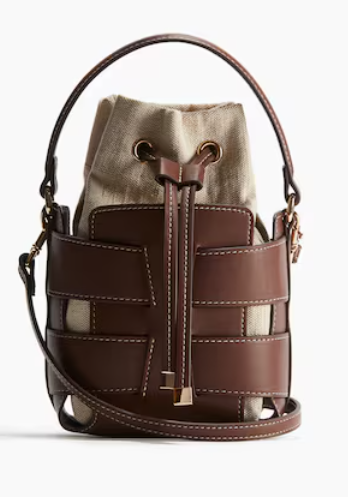
\includegraphics[width=3cm]{d66263bfc01a4e24a5536c6c8811c284.png}};
  \end{tikzpicture}

  \vspace{3mm}
  {\color{black}\LARGE \textbf{Pape Saliou FALL}}

  \vspace{1mm}
  {\large Ingénieur Data Scientist \& Développeur IA}

  \vspace{3mm}
  {\color{gray}\rule{\linewidth}{0.4pt}} \\
\end{minipage}

% ── Coordonnées
\begin{tabular}{@{}c l}
  \faPhone &
  \begin{tabular}[t]{@{}l@{}}
    {\color{gray}Téléphone} \\ 0753481453
  \end{tabular} \\
  \\
  \faLinkedin &
  \begin{tabular}[t]{@{}l@{}}
    {\color{gray}LinkedIn} \\
    \href{@pape-saliou-fall-43154a211/}{}
  \end{tabular} \\
  \\
  \faMapMarker &
  \begin{tabular}[t]{@{}l@{}}
    {\color{gray}Adresse} \\ 95300 Pontoise \\ 
  \end{tabular} \\
  \\
  \faEnvelope &
  \begin{tabular}[t]{@{}l@{}}
    {\color{gray}Email} \\
    \href{mailto:papesalioufall2@gmail.com}{papesalioufall2@gmail.com}
  \end{tabular} \\
\end{tabular}

\vspace{2mm}
{\color{gray}\rule{\linewidth}{0.4pt}} \\

% ── Langues --------------------------------------------------------
{\color{black}{Langues}}

\vspace{2mm}
\begin{itemize}[leftmargin=*]
\item Français - \textcolor{gray}{Natif}
\item Anglais - \textcolor{gray}{B2}\end{itemize}          % ← le placeholder va contenir \begin{itemize}…\end{itemize}

{\color{gray}\rule{\linewidth}{0.4pt}} \\

% ── Compétences ----------------------------------------------------
\vspace{2mm}
{\color{black}{Compétences Clés}}

\vspace{2mm}
\begin{itemize}[leftmargin=*]
\item Python
\item SQL
\item MachineLearning
\item DeepLearning
\item PowerBI
\item Git
\item NLP\end{itemize}              % ← idem, une vraie liste
\vspace{2mm}
{\color{gray}\rule{\linewidth}{0.4pt}} \\

% ── Centres d'intérêt
\vspace{2mm}
{\color{black}{Centres d’intérêt}}

\vspace{2mm}
\begin{itemize}[leftmargin=*]
\item Lecture \& veille technologique
\item Randonnée / sports outdoor
\item Voyages \& découverte culturelle
\end{itemize}     % ← simple itemize ou tabular

\vfill
~

% ────────────────────────────────────────
\switchcolumn
% Colonne droite
% ────────────────────────────────────────
\color{black}

% ── Profil
\textcolor{black}{\Large \textbf{Profil Professionnel}} \\[2pt]
Data Scientist confirmé, je conçois et déploie des solutions d’intelligence artificielle transformant des données complexes en leviers opérationnels. Autonome et force de proposition, j’assure la mise en production de modèles prédictifs robustes et l’automatisation des processus analytiques. Habitué au travail en équipe, je privilégie les environnements dynamiques où l’innovation et l’excellence sont centrales. Mon objectif est de relever de nouveaux défis techniques tout en créant de la valeur tangible pour l’entreprise. \\[8pt]

% ── Expérience
\textcolor{black}{\Large \textbf{Expérience Professionnelle}} \\[2pt]

\colorbox{maincolor}{%
  \begin{minipage}{\linewidth}
    \textbf{Data Scientist \& Développeur IA} \\ Prepaya \\ 01/2024 - Présent
    \begin{itemize}
      \item Conçu et déployé une plateforme IA avec Python/Flask, rendant les modèles prédictifs accessibles aux équipes métier. \item Implémenté des algorithmes de machine / deep learning pour l’analyse de séries temporelles, augmentant la précision des prévisions. \item Géré PostgreSQL et Heroku, intégré l’API OpenAI et automatisé les flux de données pour accélérer les cycles d’itération.
    \end{itemize}
  \end{minipage}}

\vspace{3mm}


\colorbox{maincolor}{%
  \begin{minipage}{\linewidth}
    \textbf{Apprenti Risk Analyst \& Data Scientist} \\ AXA XL \\ 12/2022 - 12/2023
    \begin{itemize}
      \item Automatisé la collecte de données financières via scripts Python/VBA, divisant par deux le temps de reporting. \item Développé des tableaux de bord Power BI pour Finance et Management, améliorant la visibilité sur la facturation. \item Créé un modèle de prédiction de sinistres en Python/R, contribuant à une meilleure évaluation du risque client.
    \end{itemize}
  \end{minipage}}

\vspace{3mm}


\colorbox{maincolor}{%
  \begin{minipage}{\linewidth}
    \textbf{Apprenti Data Scientist} \\ Prepaya \\ 09/2021 - 08/2022
    \begin{itemize}
      \item Élaboré des modèles NLP (BERT, T5) pour générer automatiquement des formulaires, réduisant le temps de création. \item Réalisé une analyse de sentiments sur les avis clients, fournissant des recommandations d’amélioration du service. \item Automatisé le scraping et le nettoyage de données avec BeautifulSoup/Selenium, garantissant la qualité des jeux de données.
    \end{itemize}
  \end{minipage}}   % ← blocs \colorbox{maincolor}{\begin{minipage}…}

\vspace{8mm}

% ── Formation
\textcolor{black}{\Large \textbf{Formation}} \\[2pt]

    \begin{tabularx}{\linewidth}{@{}c X@{}}
    \textcolor{sidetext}{\faGraduationCap} &
    \textbf{Master 2 Data Science} \\
    & Sorbonne Université \\
    & \begin{itemize}[leftmargin=*]
  \item Approfondissement en analyse de données, apprentissage automatique et deep learning. \item Projets appliqués sur séries temporelles, bases de données et calcul parallèle. \item Formation à la modélisation statistique avancée et aux structures latentes.
\end{itemize} \\
    & \textit{09/2021 - 03/2022}
    \end{tabularx}
           % ← lignes tabular par diplôme

\end{paracol}
\end{document}

